\subsubsection{Tacotron 2}
Tacotron 2 is a deep neural sequence-to-sequence model that generates mel spectrograms from text. 
I can be combined with a deep neural vocoder, it forms an end-to-end text-to-speech system.
\subsubsection{WaveGlow}
%https://medium.com/subex-ai-labs/understanding-normalizing-flows-and-its-use-case-in-speech-synthesis-part-1-5f805c2d43ce
%https://medium.com/subex-ai-labs/understanding-normalizing-flows-and-its-use-case-in-speech-synthesis-part-2-3e19840e80b5
%https://www.youtube.com/watch?v=B3WlTVvdI5M
%
WaveGlow is a deep neural vocoder that generates waveform audio from mel spectrograms \citep{waveglow}. It has a 
flow-based architecture that learns an invertible mapping, converting a noise vector and 
additional conditioning input into nearly human-sounding waveform audio. Its audio generation 
is accomplished by sampling from a distribution, which is transformed as it passes through the model 
and is conditioned on mel-spectrograms representing the audio that is to be output in waveform.

It is based on the Glow architecture for image generation \citep{glow} and on WaveNet, the groundbreaking 
autoregressive waveform generation model \citep{wavenet}. Its primary advantage over WaveNet is faster inference speed;
because it is non-autoregressive, it can generate audio much faster than WaveNet, and 25 times faster 
than real time on a V100 GPU [XX].

%Its basic architecture is illustrated below:\\
%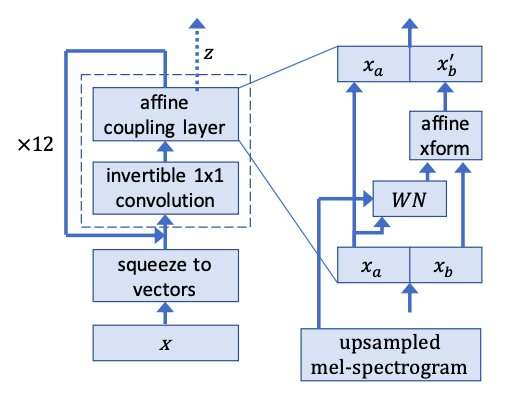
\includegraphics[width=15cm]{img/img_waveglow.jpg}

%Note that much of the computational work is done repetitively, the convolutional and subsequent 
%affine coupling layer are repeated 12 times to generate the level of fine-grained detail 
%required in high-quality waveform.


\subsubsection{CycleGAN}
As described above, in `vanilla' Generative Adversarial Networks, the input is typically random noise, which is mapped to some point in the 
target distribution. Moreover, because the generator is rewarded simply for generating some output 
appearing to have been drawn from the target distribution, there is no direct control over which 
point from the target distribution is generated.
However, there are many applications in which one might wish to exert more control over the output 
by conditioning on some desired criteria. One common case involves the task of image translation,
in which certain aspects of an image are altered while others remain intact. A simple example of 
image translation is a model that transforms horses into zebras. In this case, a simple GAN may take 
a horse image as input and output a very dissimilar zebra image as output; this is because there 
is no constraint to enforce content preservation.
CycleGAN \citep{cycleganvc} achieves this by training an inverse generator to map the transformed image back to the 
original. This cyclical consistency constraint requires the forward generator to preserve semantic 
content from the original image so that it the original can be reconstructed from the transformed image.

\subsubsection{MelGAN-VC}
Most work on GANs focuses on data with a fixed output shape, where 
input size and output shape are typically equal, such as in the case of image generation. 
When an input is supplied, it is for the purpose of conditioning the output and the input 
typically has the same shape as the output.

In settings where the data has an intrinsically sequential nature and the input size varies, 
it is not possible to require a fixed and shape. One such setting is voice conversion, and one 
simple and effective solution has been proposed by Marco Pasini in [XX], illustrated below:\\
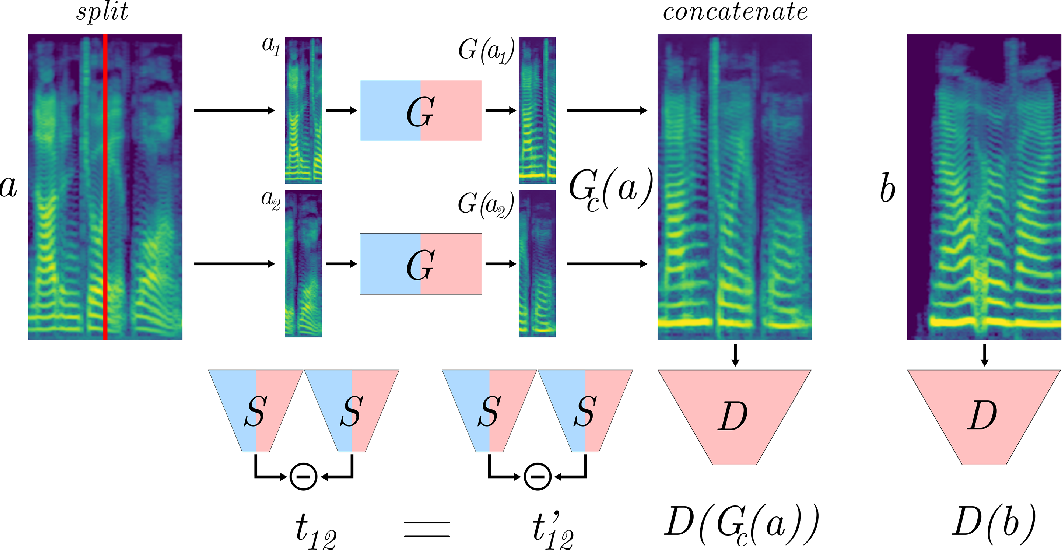
\includegraphics[width=\textwidth]{img/img_melganvc.png}

The key insight is that by taking a fixed length ($T$ frames) of the input spectrogram, 
then splitting the input into two equal-sized blocks and passing each to the generator network. 
The converted spectrograms, i.e. the two generator outputs are then recombined and passed 
to the discriminator. Due to the adversarial loss training objective, the generator must learn 
to convert each block in such a way that, when reassembled, it will be indistinguishable from 
a real sample from the target set. Because the target set does not contain spectrograms with 
discontinuities, such a discontinuity at the splitting point would clearly identify a fake sample. 
Thus, the generator is incentivized to produce outputs which, when re-joined, do not contain 
such telltale discontinuities at the splitting points. Because this applies to any  split point, 
it is possible to train a relatively small generator that can receive inputs of arbitrarily length 
one block at a time and generate the desired output.

\iffalse
\subsubsection{Reinforcement learning and the REINFORCE Algorithm}
Reinforcement learning is a paradigm of machine learning that is well-suited to settings in which an agent 
interacts with an environment and receives rewards as a function of its actions. The objective is to 
choose actions so as to maximize long-term reward. Thus, reinforcement learns a policy, a mapping from 
state to action. The optimal policy yields the maximum expected long-term reward.

There are several different families of approaches in reinforcement learning. 

The REINFORCE algorithm  

\subsubsection{SeqGAN and StepGAN [2]}
Soon after their initial introduction in 2014, GANs achieved remarkable successes in image generation. 
Unfortunately, the GAN framework proved somewhat more difficult to apply to natural language, primarily 
because its gradient-based methods do not work for discrete-valued sequences. To remedy this, 
XXX introduced SeqGAN, an adaptation of GANs to the setting of discrete-valued sequences.

SeqGAN uses the REINFORCE algorithm for training. 
\fi

\subsubsection{Allosaurus}
Allosaurus is a Python library containing tools for automatic neural phonetic transcriptions 
using IPA \Citep{allosaurus}.
Released by a team of researchers at Carnegie Mellon University, it performs phone recognition, 
rather than the more typical task of phoneme recognition, and its main innovation is its so-called 
``allophone layer''. This is a phone-to-phoneme mapping that restricts the phonetic invntory to 
that of a single language. This enable Allosaurus to capture the benefits both of shared phoneme 
models and private phoneme models. While all three architectures use an encoder, shared phoneme models 
use a common phone layer across languages, while in the private phoneme model, each language 
has a separate model following the shared encoder. Allosaurus strikes a balance by using a shared 
decoder or ``universal phone layer'' and leaving the per-language customization to the allophone layer. 
This allows the decoder to benefit from larger amounts of training data and greater generality.
These differences in architecture are shown below:
\begin{center}
  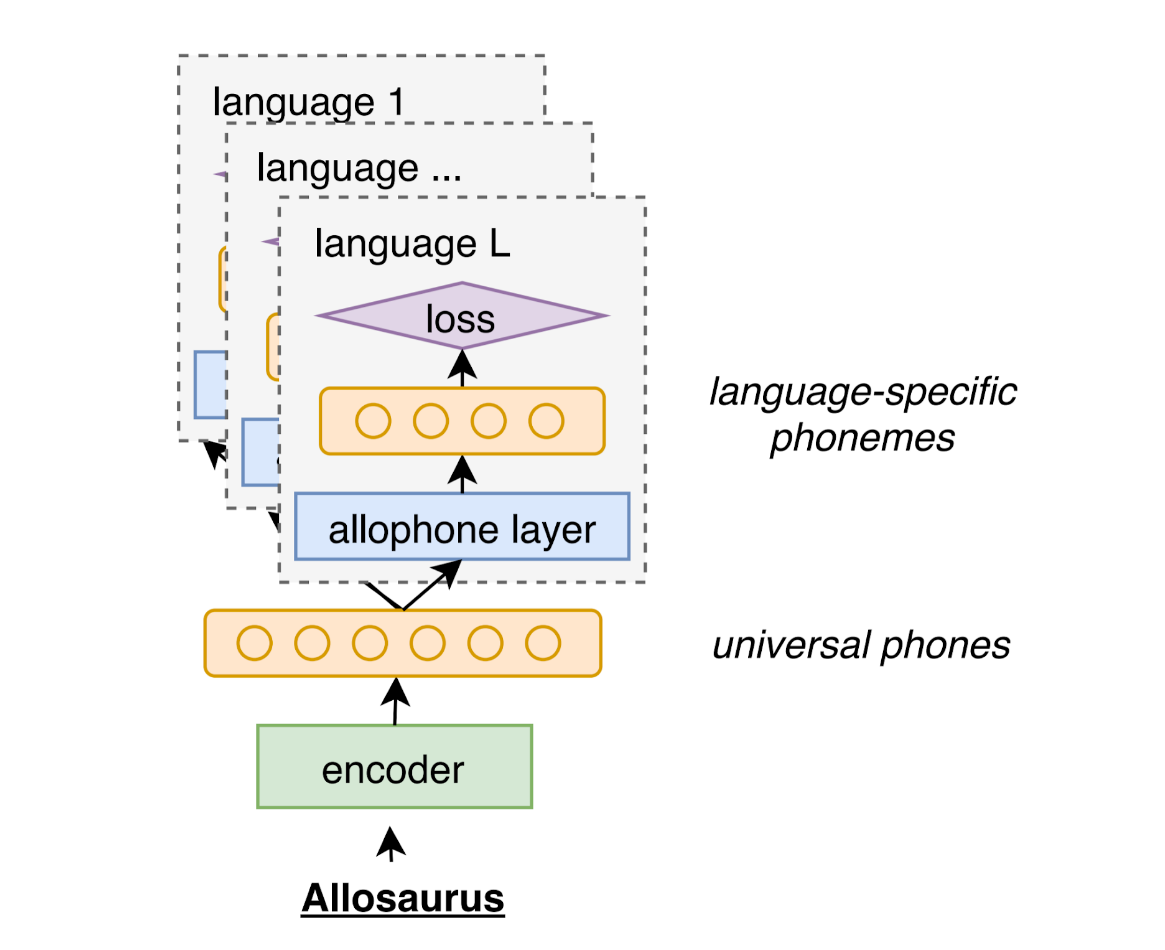
\includegraphics[width=7cm]{img/img_alloraurus.png}
\end{center}

\cite{ctc}

%http://www.scholarpedia.org/article/Policy_gradient_methods#Likelihood_Ratio_Methods_and_REINFORCE
%http://www.scholarpedia.org/article/Policy_gradient_methods#Likelihood_Ratio_Methods_and_REINFORCE
%https://lilianweng.github.io/lil-log/2018/02/19/a-long-peek-into-reinforcement-learning.html
%https://lilianweng.github.io/lil-log/2018/04/08/policy-gradient-algorithms.html
%https://www.quora.com/What-is-the-REINFORCE-algorithm
%
%
%
%